\chapter{AFML: Backtesting with Triple Barriers and Purged CV}
\label{ch:afml}

\begin{companioncode}{quant-backtest}
Code: \texttt{crates/quant-backtest/}\\
Dependencies: \crate{quant-core}, \crate{quant-timeseries}, \crate{quant-portfolio}, \crate{thiserror}\\
Run: \texttt{cargo run -p quant-backtest --example triple\_barrier}\\
Run: \texttt{cargo run -p quant-backtest --example purged\_cv}\\
Run: \texttt{cargo run -p quant-backtest --example kelly\_sizing}
\end{companioncode}

\section{Learning Objectives}

This chapter leaves behind the frictionless world of portfolio theory
and the single-trade world of microstructure, and enters the engine
room of systematic strategy research: how do you train a model on
time-series labels, cross-validate it without leaking information, and
size the resulting bets? After completing it you can:

\begin{itemize}
    \item Explain why standard k-fold cross-validation leaks
      information on financial time series with overlapping events
    \item Label a price series with the triple-barrier method
      (profit-taking, stop-loss, time barrier) and convert the labels
      to a binary outcome
    \item Compute the concurrency of overlapping events and derive
      sample weights from event uniqueness
    \item Generate purged k-fold splits with an embargo period that
      removes training samples overlapping --- and immediately
      following --- each test fold
    \item Compute the full Kelly criterion from a win probability and
      a win/loss ratio, and apply a fractional multiplier for risk
      control
    \item Run the end-to-end AFML pipeline that combines all of the
      above into a single backtest report
\end{itemize}

\begin{keyinsight}
Traditional backtesting fails on three fronts: labels are arbitrary
(fixed-horizon return sign), samples overlap (events that span
multiple bars share information), and cross-validation leaks (the
test fold is not independent of the training fold). The AFML framework
fixes all three: triple-barrier labels are path-dependent, sample
weights discount overlap, and purged k-fold with embargo removes
leakage. The result is an out-of-sample Sharpe that you can actually
trust.
\end{keyinsight}

\section{Why Traditional Backtesting Fails}

A naive backtest labels each bar by the sign of the return over a
fixed horizon $h$ --- for example, the 5-bar forward return --- and
trains a classifier on those labels. Three problems compound:

\begin{enumerate}
    \item \textbf{Arbitrary labels.} A 5-bar forward return says
      nothing about the path: a position that gained 4\%, lost 3\%,
      and gained 4\% again is labelled the same as one that monotonically
      drifted up. Yet the lived experience of holding the position
      is very different --- the first path probably hit a stop loss.
    \item \textbf{Overlapping samples.} Consecutive 5-bar labels share
      four of their five bars. A classifier that treats them as
      independent over-counts the information in the sample by a factor
      of $\sim h$, inflating the apparent edge.
    \item \textbf{Leakage in CV.} Standard k-fold CV assigns bars to
      folds uniformly at random. A training bar that is part of a
      5-bar event ending inside the test fold has already seen the
      label of that test sample --- the validation is no longer
      out-of-sample.
\end{enumerate}

The AFML framework of López de Prado (2018) addresses each in turn.

\section{The Triple-Barrier Method}

For each entry point $t_0$ the method places three barriers around
the entry price $P_{t_0}$:

\begin{itemize}
    \item \textbf{Upper} at $P_{t_0}(1 + \theta^+)$, the
      profit-taking threshold.
    \item \textbf{Lower} at $P_{t_0}(1 + \theta^-)$, the
      stop-loss threshold ($\theta^- < 0$).
    \item \textbf{Time} at $t_0 + T$, the maximum holding period.
\end{itemize}

We walk the price path forward from $t_0$ and label the event by
the \emph{first} barrier touched. The holding period is the number of
bars from entry to exit; the return is $(P_{\text{exit}} -
P_{t_0})/P_{t_0}$.

\begin{marginfigure}
    \centering
    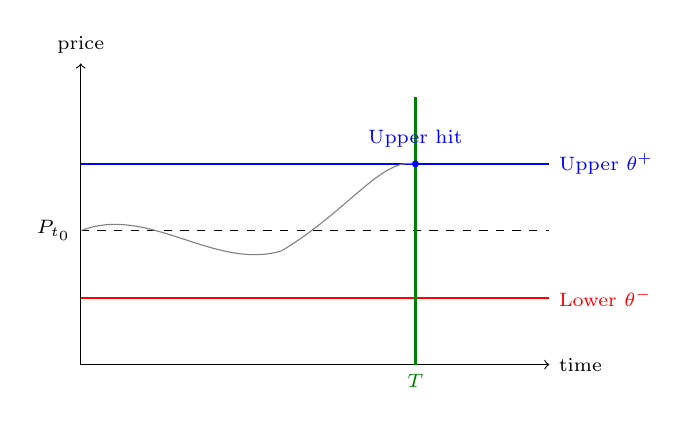
\begin{tikzpicture}[scale=0.85, font=\scriptsize]
        % Price axis
        \draw[->] (0,0) -- (7,0) node[right] {time};
        \draw[->] (0,0) -- (0,4.5) node[above] {price};
        % Entry
        \draw[dashed] (0,2) -- (7,2);
        \node[left] at (0,2) {$P_{t_0}$};
        % Upper barrier
        \draw[blue, thick] (0,3) -- (7,3);
        \node[blue, right] at (7,3) {Upper $\theta^+$};
        % Lower barrier
        \draw[red, thick] (0,1) -- (7,1);
        \node[red, right] at (7,1) {Lower $\theta^-$};
        % Time barrier
        \draw[green!50!black, thick] (5,0) -- (5,4);
        \node[green!50!black, below] at (5,0) {$T$};
        % Price path
        \draw[gray] (0,2) .. controls (1,2.4) and (2,1.4) .. (3,1.7);
        \draw[gray] (3,1.7) .. controls (4,2.3) and (4.5,3.1) .. (5,3);
        \fill[blue] (5,3) circle (1.5pt);
        \node[blue, above] at (5,3.1) {Upper hit};
    \end{tikzpicture}
    \caption{Triple barriers around the entry price. The first
    barrier touched --- here the upper barrier at time $T$ ---
    determines the label.}
    \label{fig:triple-barrier}
\end{marginfigure}

\subsection{Configuration and Labels}

\marginnote{%
\textbf{Why three barriers?}\\[0.3em]
A path-dependent label captures the lived experience of the trade.
Two trades with the same 5-bar return but different paths get
different labels: one hits the upper barrier (a win), the other
hits the stop loss (a loss). The label is no longer a function of
the endpoint, but of the whole trajectory.
}

\begin{lstlisting}[caption={Triple-barrier configuration and label type}]
pub struct TripleBarrierConfig {
    pub upper_barrier: f64, // e.g. 0.02 = +2%
    pub lower_barrier: f64, // e.g. -0.02 = -2%
    pub time_barrier: usize, // max bars to hold
    pub min_return: f64, // threshold for Time label
}

pub enum TripleBarrierLabel { Upper, Lower, Time }

pub struct LabeledEvent {
    pub entry_index: usize,
    pub exit_index: usize,
    pub label: TripleBarrierLabel,
    pub return_pct: f64,
    pub holding_period: usize,
}
\end{lstlisting}

\subsection{Labeling a Single Event}

\func{label\_one} walks prices forward from the entry index, checking
at each bar whether the upper or lower barrier has been hit. If neither
is touched before the time barrier expires, the event is labelled
\texttt{Time} with the return at the last bar.

\marginnote{%
\textbf{No look-ahead in features}\\[0.3em]
The triple-barrier method \emph{intentionally} uses future prices to
label the event. That is not look-ahead bias in the model: the label
is the target, not a feature. Features must be computed strictly
from information available at $t_0$. The discipline is: train on
labels that depend on the future, predict them from features that
do not.
}

\begin{lstlisting}[caption={Walking the price path to find the first barrier hit}]
fn label_one(prices: &[f64], entry_index: usize,
             config: &TripleBarrierConfig) -> Result<LabeledEvent, BacktestError> {
    let p_entry = prices[entry_index];
    let upper_px = p_entry * (1.0 + config.upper_barrier);
    let lower_px = p_entry * (1.0 + config.lower_barrier);
    let last = (entry_index + config.time_barrier).min(prices.len() - 1);
    for (t, &p) in prices.iter().enumerate()
        .take(last + 1).skip(entry_index + 1) {
        if p >= upper_px {
            return Ok(LabeledEvent {
                entry_index, exit_index: t,
                label: TripleBarrierLabel::Upper,
                return_pct: (p - p_entry) / p_entry,
                holding_period: t - entry_index,
            });
        }
        if p <= lower_px {
            return Ok(LabeledEvent {
                entry_index, exit_index: t,
                label: TripleBarrierLabel::Lower,
                return_pct: (p - p_entry) / p_entry,
                holding_period: t - entry_index,
            });
        }
    }
    let p_exit = prices[last];
    Ok(LabeledEvent {
        entry_index, exit_index: last,
        label: TripleBarrierLabel::Time,
        return_pct: (p_exit - p_entry) / p_entry,
        holding_period: last - entry_index,
    })
}
\end{lstlisting}

\subsection{Binary Labels}

For a long-only strategy the label is naturally binary: Upper is a
win (1), Lower is a loss (0), and Time is a win iff the return at
the time barrier exceeds $\theta^+_{\min}$.

\begin{lstlisting}[caption={Converting a triple-barrier label to a binary outcome}]
pub fn to_binary_label_helper(label: TripleBarrierLabel,
                              event: &LabeledEvent,
                              min_return: f64) -> i32 {
    match label {
        TripleBarrierLabel::Upper => 1,
        TripleBarrierLabel::Lower => 0,
        TripleBarrierLabel::Time => {
            if event.return_pct >= min_return { 1 } else { 0 }
        }
    }
}
\end{lstlisting}

\section{Sample Uniqueness and Weighting}

When events overlap in time, each carries less unique information. A
training sample whose event $[t_0, t_1]$ shares all of its bars with
three other events is worth roughly a third of a sample that no other
event touches. We capture this with the concurrency count
$c_t$ = number of events active at bar $t$:

\begin{equation}
    c_t = \sum_i \mathbb{1}_{[t_0^{(i)},\, t_1^{(i)}]}(t).
\end{equation}

The average uniqueness of event $i$ is the mean of $1/c_t$ over its
duration, and the sample weight is the inverse of the average
concurrency:

\begin{equation}
    u_i = \frac{1}{t_1^{(i)} - t_0^{(i)}} \sum_{t=t_0^{(i)}}^{t_1^{(i)}} \frac{1}{c_t},
    \qquad
    w_i = \frac{1}{\bar{c}_i}.
\end{equation}

\marginnote{%
\textbf{Why inverse concurrency?}\\[0.3em]
If three events overlap on a bar, each one contributes a third of
the unique information there. Summing $1/c_t$ over the duration
averages that discount across the event's life. The resulting
weight is high for isolated events and low for crowded ones, so
the classifier down-weights redundant samples automatically.
}

\begin{lstlisting}[caption={Concurrency counts and average uniqueness}]
pub fn concurrent_events(events: &[LabeledEvent], n_bars: usize) -> Vec<usize> {
    let mut counts = vec![0usize; n_bars];
    for ev in events {
        let start = ev.entry_index.min(n_bars);
        let end = ev.exit_index.min(n_bars.saturating_sub(1));
        if start >= n_bars { continue; }
        for c in counts.iter_mut().take(end + 1).skip(start) { *c += 1; }
    }
    counts
}

pub fn average_uniqueness(events: &[LabeledEvent], n_bars: usize) -> Vec<f64> {
    let concurrent = concurrent_events(events, n_bars);
    events.iter().map(|ev| {
        let start = ev.entry_index;
        let end = ev.exit_index.min(n_bars.saturating_sub(1));
        if end < start { return 0.0; }
        let mut sum_inv = 0.0;
        let mut count = 0;
        for &c in concurrent.iter().take(end + 1).skip(start) {
            if c > 0 { sum_inv += 1.0 / c as f64; count += 1; }
        }
        if count == 0 { 0.0 } else { sum_inv / count as f64 }
    }).collect()
}
\end{lstlisting}

The final weights are the inverse of the average concurrency during
each event, normalised to sum to one across the sample:

\begin{lstlisting}[caption={Sample weights from inverse concurrency}]
pub fn sample_weights(events: &[LabeledEvent], n_bars: usize) -> Vec<f64> {
    let concurrent = concurrent_events(events, n_bars);
    let mut weights: Vec<f64> = events.iter().map(|ev| {
        let start = ev.entry_index;
        let end = ev.exit_index.min(n_bars.saturating_sub(1));
        if end < start { return 0.0; }
        let mut sum_c = 0.0;
        let mut count = 0;
        for &c in concurrent.iter().take(end + 1).skip(start) {
            if c > 0 { sum_c += c as f64; count += 1; }
        }
        if count == 0 { 0.0 } else { 1.0 / (sum_c / count as f64) }
    }).collect();
    let total: f64 = weights.iter().sum();
    if total > 0.0 { for w in &mut weights { *w /= total; } }
    weights
}
\end{lstlisting}

\section{Purged K-Fold Cross-Validation}

Standard k-fold CV leaks information whenever a training event
overlaps a test event. \emph{Purging} removes from the training
fold any event whose $[t_0, t_1]$ interval intersects the test fold
$[t_{\text{start}}, t_{\text{end}})$.

\begin{lstlisting}[caption={Overlap test for purging}]
pub fn event_overlaps(event: &LabeledEvent, start: usize, end: usize) -> bool {
    event.entry_index < end && event.exit_index > start
}
\end{lstlisting}

\marginnote{%
\textbf{Train must not see test}\\[0.3em]
If a training event ends inside the test window, its label ---
which depends on prices inside the test window --- has already
told the model what happens there. Purging removes exactly those
events, leaving the training fold honest.
}

\subsection{Embargo}

Purging is not enough under autocorrelation: a training event
\emph{starting} just after the test window ends still carries
test-window information through serially-correlated features. The
\emph{embargo} removes training events whose entry falls in
$[t_{\text{end}}, t_{\text{end}} + e)$.

\begin{lstlisting}[caption={Purged k-fold with embargo}]
pub fn purged_kfold_splits(events: &[LabeledEvent], n_bars: usize,
                           config: &PurgedKFoldConfig) -> Vec<PurgedSplit> {
    let fold_size = n_bars / config.n_folds;
    let mut splits = Vec::with_capacity(config.n_folds);
    for k in 0..config.n_folds {
        let t_start = k * fold_size;
        let t_end = if k == config.n_folds - 1 { n_bars }
                    else { (k + 1) * fold_size };
        let embargo_end = (t_end + config.embargo).min(n_bars);
        let mut train = Vec::new();
        let mut test = Vec::new();
        let mut purged = 0usize;
        let mut embargoed = 0usize;
        for (i, ev) in events.iter().enumerate() {
            if ev.entry_index >= t_start && ev.entry_index < t_end {
                test.push(i); continue;
            }
            if event_overlaps(ev, t_start, t_end) { purged += 1; continue; }
            if ev.entry_index >= t_end && ev.entry_index < embargo_end {
                embargoed += 1; continue;
            }
            train.push(i);
        }
        splits.push(PurgedSplit {
            train_indices: train, test_indices: test,
            purged_count: purged, embargoed_count: embargoed,
        });
    }
    splits
}
\end{lstlisting}

\marginnote{%
\textbf{Embargo calibrates autocorrelation}\\[0.3em]
Set the embargo to the lag at which the autocorrelation function
of the features drops below significance. For daily returns on
liquid equities a 1--5 bar embargo is typical; for noisy
high-frequency features a longer embargo is needed. An embargo of
zero reduces to plain purging.
}

\section{Bet Sizing: The Kelly Criterion}

A good label tells you \emph{when} to bet; it does not tell you
\emph{how much}. The Kelly criterion maximises the expected log
growth of capital. For a binary bet with win probability $p$, loss
probability $q = 1 - p$, and win/loss ratio $b = \bar{r}^+ /
|\bar{r}^-|$ (mean win divided by mean loss), the optimal fraction
of capital to risk on each bet is

\begin{equation}
    f^* = \frac{p\, b - q}{b} = p - \frac{q}{b}.
    \label{eq:kelly}
\end{equation}

The criterion is exact for a sequence of i.i.d.\ bets with
known parameters. In practice the parameters are estimated, so
\emph{fractional Kelly} --- using a fraction $\lambda \in (0, 1]$ of
$f^*$ --- is standard. Half Kelly ($\lambda = 0.5$) achieves most of
the growth with roughly half the variance.

\marginnote{%
\textbf{Kelly in one line}\\[0.3em]
$f^*$ is the edge divided by the odds. With no edge ($p = q =
0.5$, $b = 1$) it is zero --- you bet nothing. With a 60\% win
rate and 1:1 payoff it is $0.6 - 0.4 = 0.2$: risk 20\% of capital
per bet. Beyond that, the variance of log-wealth grows faster
than its mean.
}

\begin{lstlisting}[caption={Kelly criterion and fractional variant}]
pub fn kelly_fraction(win_prob: f64, win_loss_ratio: f64) -> f64 {
    let q = 1.0 - win_prob;
    win_prob - q / win_loss_ratio
}

pub fn fractional_kelly(win_prob: f64, win_loss_ratio: f64, fraction: f64) -> f64 {
    kelly_fraction(win_prob, win_loss_ratio) * fraction
}
\end{lstlisting}

To estimate Kelly from historical trade returns, compute the win
probability as the fraction of positive trades and the win/loss ratio
as the mean win divided by the mean loss:

\begin{lstlisting}[caption={Kelly from a series of trade returns}]
pub fn kelly_from_returns(returns: &[f64]) -> f64 {
    let n = returns.len() as f64;
    let wins: Vec<f64> = returns.iter().copied().filter(|&r| r > 0.0).collect();
    let losses: Vec<f64> = returns.iter().copied().filter(|&r| r < 0.0).collect();
    let p = wins.len() as f64 / n;
    let mean_win = wins.iter().sum::<f64>() / wins.len().max(1) as f64;
    let mean_loss = -losses.iter().sum::<f64>() / losses.len().max(1) as f64;
    if mean_loss <= 0.0 { return 0.0; }
    kelly_fraction(p, mean_win / mean_loss)
}
\end{lstlisting}

\subsection{Position Sizing}

The \func{compute\_position\_size} helper packages full and half Kelly
along with the empirical win probability and win/loss ratio so the
backtest can switch sizing rules without recomputing statistics.

\begin{lstlisting}[caption={Position sizing summary}]
pub struct PositionSize {
    pub kelly_full: f64,
    pub kelly_half: f64,
    pub win_probability: f64,
    pub win_loss_ratio: f64,
}

pub fn compute_position_size(trade_returns: &[f64]) -> PositionSize {
    let n = trade_returns.len() as f64;
    let wins: Vec<f64> = trade_returns.iter().copied().filter(|&r| r > 0.0).collect();
    let losses: Vec<f64> = trade_returns.iter().copied().filter(|&r| r < 0.0).collect();
    let p = wins.len() as f64 / n.max(1) as f64;
    let mean_win = wins.iter().sum::<f64>() / wins.len().max(1) as f64;
    let mean_loss = -losses.iter().sum::<f64>() / losses.len().max(1) as f64;
    let b = if mean_loss > 0.0 { mean_win / mean_loss } else { 0.0 };
    let kelly = kelly_fraction(p, b);
    PositionSize {
        kelly_full: kelly,
        kelly_half: 0.5 * kelly,
        win_probability: p,
        win_loss_ratio: b,
    }
}
\end{lstlisting}

\section{The AFML Pipeline}

The full pipeline ties the pieces together. Given a price series
and an entry step, it:

\begin{enumerate}
    \item Generates entry indices at every \texttt{entry\_step} bars.
    \item Labels each entry with the triple-barrier method.
    \item Computes sample weights from event uniqueness.
    \item Builds purged k-fold splits with embargo.
    \item Computes per-trade returns, the in-sample Sharpe, and the
      mean out-of-sample Sharpe across folds.
    \item Sizes each trade by the chosen \func{BetSizing} rule ---
      equal, full Kelly, half Kelly, or fixed fraction.
    \item Walks the trade returns through a compounded equity curve
      to compute total return and maximum drawdown.
\end{enumerate}

\begin{lstlisting}[caption={End-to-end AFML backtest}]
pub enum BetSizing { Equal, KellyFull, KellyHalf, Fixed(f64) }

pub struct AfmlBacktestConfig {
    pub barrier_config: TripleBarrierConfig,
    pub cv_config: PurgedKFoldConfig,
    pub use_weights: bool,
    pub bet_sizing: BetSizing,
    pub entry_step: usize,
}

pub struct AfmlBacktestResult {
    pub events: Vec<LabeledEvent>,
    pub weights: Vec<f64>,
    pub cv_splits: Vec<PurgedSplit>,
    pub in_sample_sharpe: f64,
    pub out_of_sample_sharpe: f64,
    pub position_size: PositionSize,
    pub total_return: f64,
    pub max_drawdown: f64,
}

pub fn afml_backtest(prices: &[f64],
                     config: &AfmlBacktestConfig)
    -> Result<AfmlBacktestResult, BacktestError>
{
    config.barrier_config.validate()?;
    // ... generate entries, label, weight, split, size, evaluate ...
    Ok(AfmlBacktestResult { ... })
}
\end{lstlisting}

\marginnote{%
\textbf{In-sample vs out-of-sample}\\[0.3em]
The in-sample Sharpe is computed on all trade returns. The
out-of-sample Sharpe is the mean of the per-fold Sharpe ratios
on each test set. A large gap between the two is the symptom of
overfitting that purged CV is designed to expose.
}

\section{Meta-Labeling (Brief)}

A primary model generates a direction signal (long/short/flat); a
secondary model --- the meta-model --- predicts whether the primary
signal will be correct. The triple-barrier label of the primary
model becomes the target of the meta-model. This separates
\emph{direction} from \emph{size}: the primary model bets often, the
meta-model decides how much to trust each bet. The result is a
betting strategy that is more selective than the primary alone and,
empirically, has a higher Sharpe.

\section{Exercises}

\begin{enumerate}
    \item \textbf{Custom barriers.} Generalise the triple-barrier
      method so that the upper and lower barriers are functions of
      rolling volatility rather than fixed percentages. How does the
      label distribution change on a noisy versus a calm series?
    \item \textbf{Embargo calibration.} Compute the autocorrelation
      function of fractional-differentiated returns (see
      \cref{ch:timeseries}) and set the embargo to the first lag
      where the ACF drops below significance. Compare the
      out-of-sample Sharpe with and without the embargo.
    \item \textbf{Volatility-scaled Kelly.} Replace the constant
      Kelly fraction with one that scales inversely with rolling
      volatility. Verify that the drawdown distribution tightens.
    \item \textbf{Meta-labeling.} Use the sign of a moving-average
      crossover as the primary signal, label it with the triple
      barrier, and train a logistic regression on the labelled events
      to predict correctness. Compare the meta-filtered strategy to
      the primary alone.
\end{enumerate}

\section{Key Takeaways}

\begin{itemize}
    \item \textbf{Triple-barrier labeling} converts price paths into
      supervised learning targets by setting profit-taking, stop-loss,
      and time barriers. It avoids the look-ahead bias of fixed-horizon
      labeling.

    \item \textbf{Sample weights from uniqueness} down-weight events
      that overlap heavily with others, reducing overfitting to
      clustered periods. The average uniqueness metric quantifies
      temporal independence.

    \item \textbf{Purged k-fold cross-validation} prevents information
      leakage by removing overlapping events from training folds and
      applying an embargo period. It exposes overfitting that standard
      k-fold misses in time-series data.

    \item \textbf{Walk-forward analysis} validates strategy robustness
      by measuring performance degradation from in-sample to
      out-of-sample. Walk-Forward Efficiency (WFE) below 0.5 indicates
      severe overfitting (see \cref{sec:walk-forward} in
      \cref{ch:backtest}).

    \item \textbf{Kelly criterion bet sizing} maximizes long-run
      geometric growth by sizing positions proportional to edge and
      inversely to volatility. Fractional Kelly trades growth for
      reduced drawdowns.

    \item \textbf{Meta-labeling} separates direction (primary model)
      from confidence (meta-model), producing more selective strategies
      with higher Sharpe ratios. The triple-barrier label of the
      primary becomes the target of the meta-model.

    \item \textbf{Trait-based architecture} enables composition of
      labeling, cross-validation, and bet sizing strategies without
      code duplication. The generic backtest engine combines any
      \texttt{Labeler}, \texttt{CrossValidator}, and \texttt{BetSizer}
      via trait bounds.

    \item \textbf{AFML workflow integration} orchestrates the full
      pipeline: label events $\to$ weight samples $\to$ cross-validate
      $\to$ size bets $\to$ evaluate. Each component is swappable via
      trait implementations, promoting experimentation and reuse.
\end{itemize}

\section{References}

\begin{itemize}
    \item López de Prado, M.\ (2018). \emph{Advances in Financial
      Machine Learning}. Wiley. Chapters 3 (triple-barrier), 4
      (sample weights), 7 (cross-validation), 10 (bet sizing).
    \item Kelly, J. L.\ (1956). ``A New Interpretation of Information
      Rate.'' \emph{Bell System Technical Journal}.
    \item \href{https://github.com/bitscrafts/quant-lab-rust}{quant-lab-rust}
      companion code, crate \crate{quant-backtest}.
\end{itemize}